\section{Study region and data}
 
\subsection{Study area}

The forest fire strategy was deployed in the VA watershed located in Colombia in the department of Antioquia (see Figure \ref{fig:ubicacion}). With an area of 1040$km^2$ with and urban development of the 40$\%$ and a population of 7M, VA houses the City of Medellin (the capital city of Antioquia) and other nine municipalities. Fires usually happen at the grasslands, small crops, and tropical vegetation located around the urban area (see critical regions Figure \ref{fig:ubicacion}).\\

\begin{figure}[h]
\centering
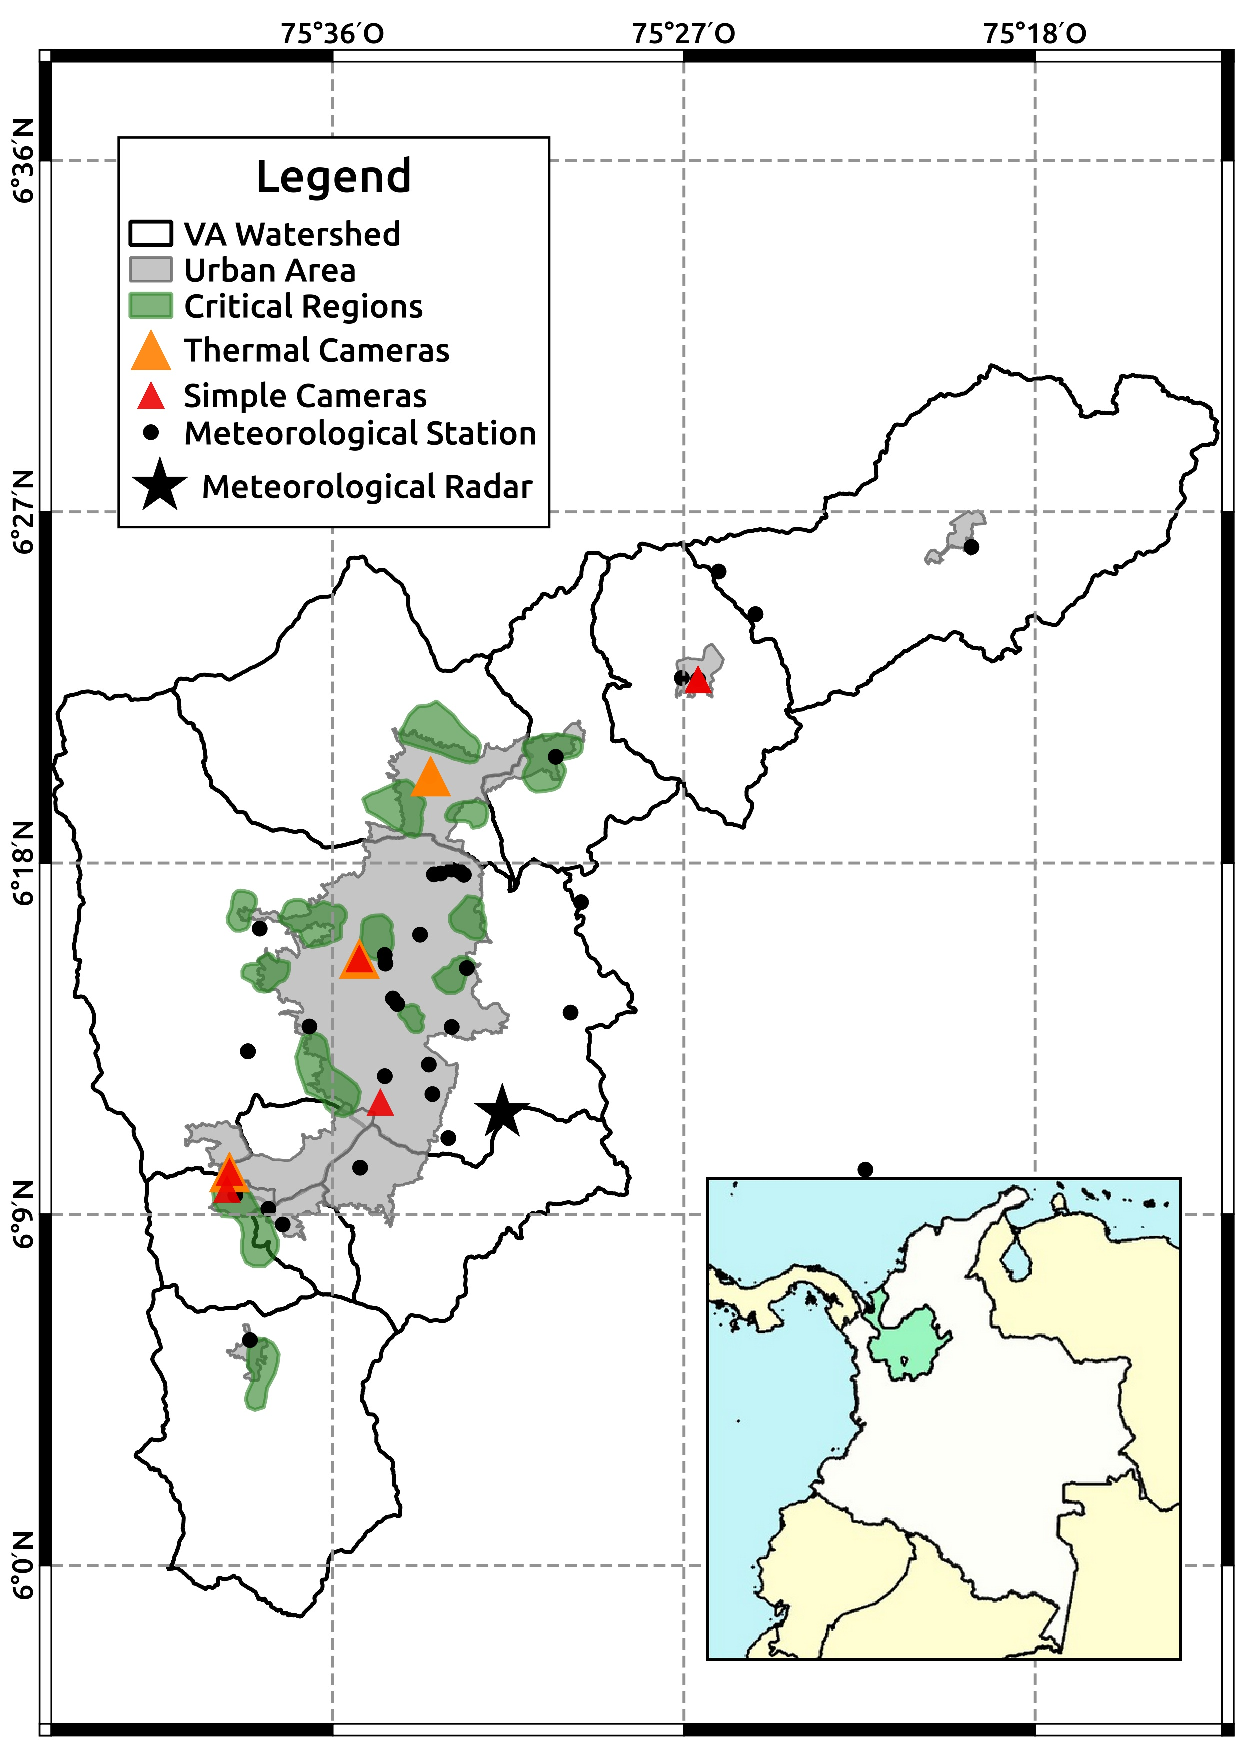
\includegraphics[trim={0.2cm 0cm 0.2cm 0cm},clip,width=8.0cm]{Figuras/map_intro_cameras.pdf}
\caption{Location Aburra Valley, critical zones for historical occurrences, high resolution cameras for monitoring and meteorological data.}
\label{fig:ubicacion}
\end{figure}

\subsection{Data}

For the fires modeling and monitoring, we use static and dynamic data.  In order to monitor 24/7, we use heat and high-definition cameras (Figure \ref{fig:ubicacion}). On the other hand, the model relies on static and dynamic raster maps data. We consider that static variables exhibit almost no change over time and are updated occasionally.  On the other hand, the dynamic variables change at each time step.\\     

The static variables consider a human interaction layer, a layer considering land use, and a layer of historical critic regions of forest fires occurrence (see Figure \ref{fig:staticLayers}). The human interaction (Figure \ref{fig:staticLayers}a) considers the vegetation fire susceptibility regardless of the climatic conditions.  These activities include urban expansion, crops expansion, roads construction, and tourism.  On the other hand, the land use layer (Figure \ref{fig:staticLayers}b) was obtained through a supervised classification of the Pleiades sensor (CITA). In this layer, we consider vegetation, grass, forest, crops, bare soil, and water bodies. Finally, the historical critic layer considers the historical occurrence of the forest fires in the last ten years.\\

\begin{figure*}
  \centering
  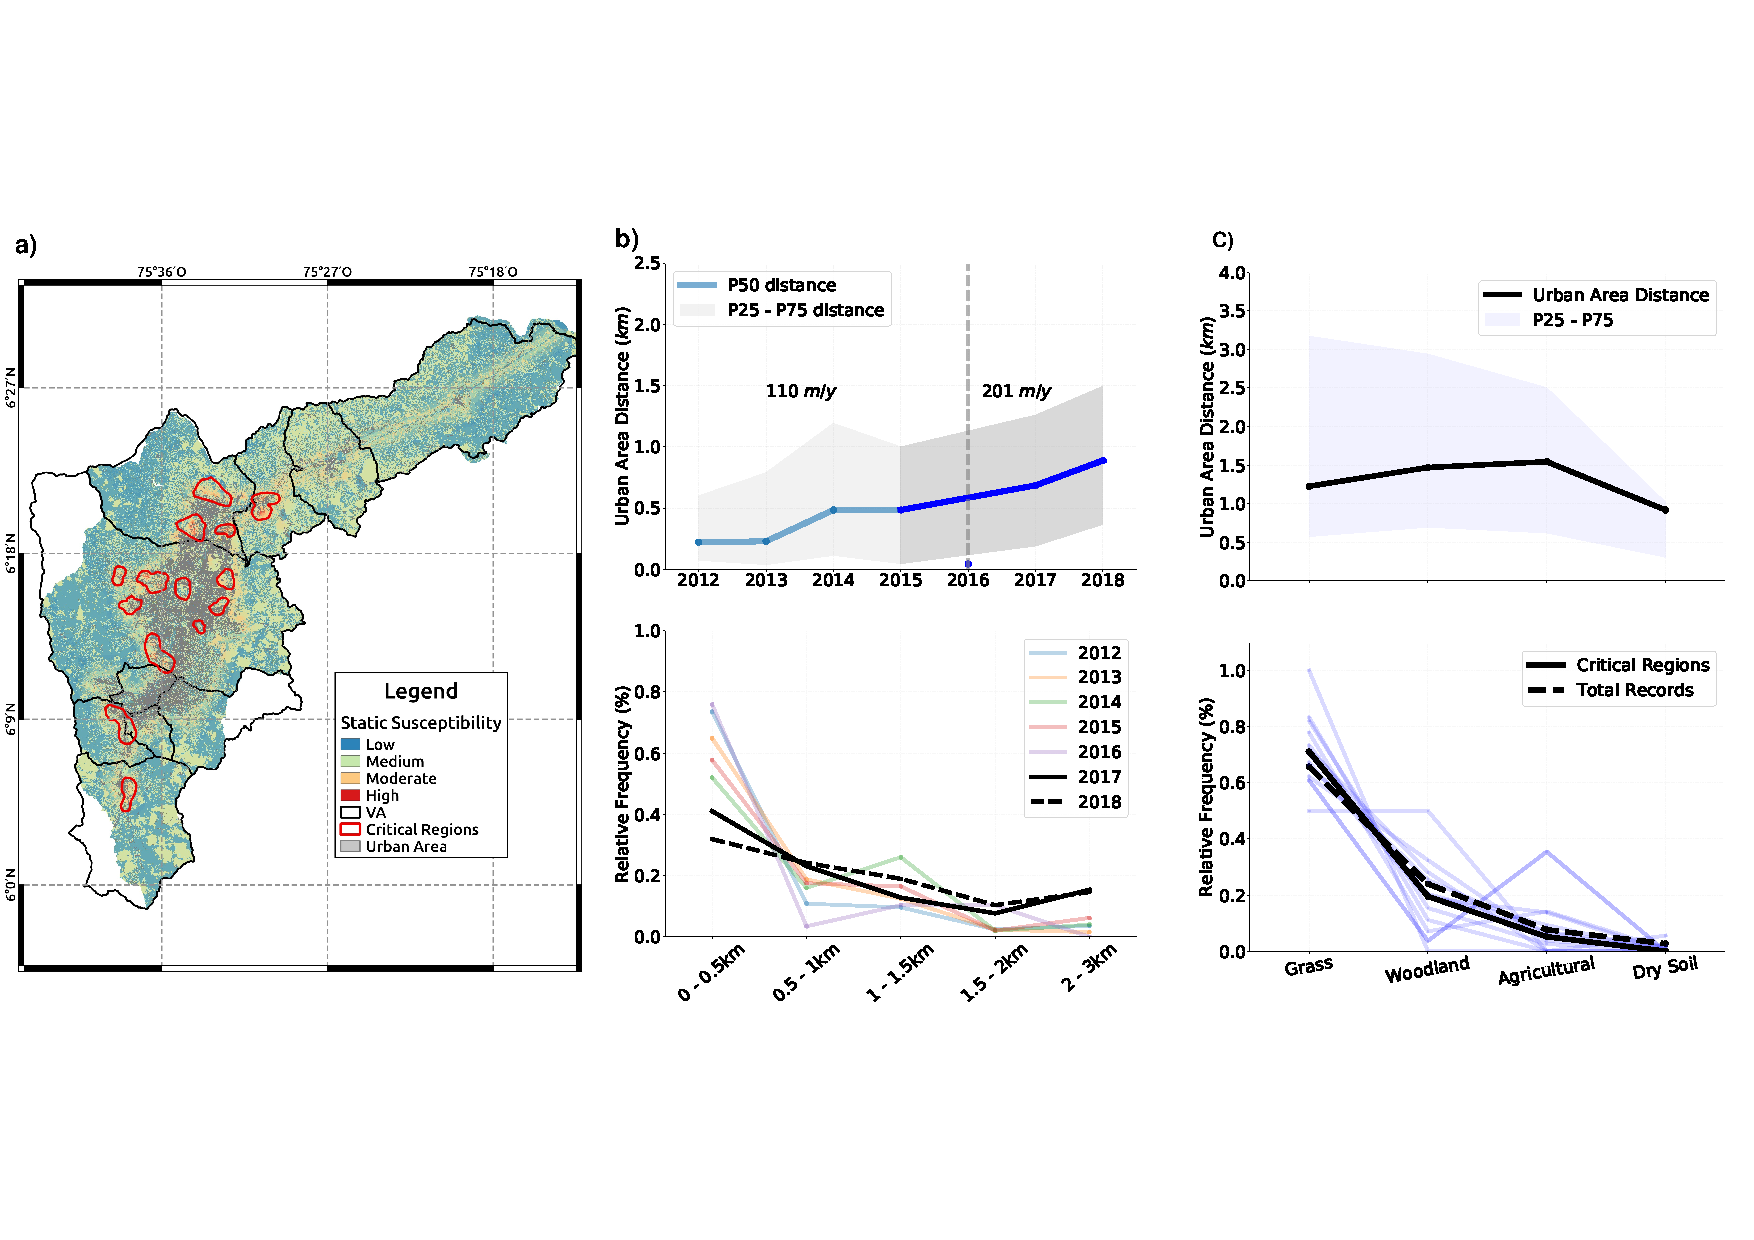
\includegraphics[width=1.0\linewidth]{Figuras/static_composition1.pdf}
  \caption{Static layer. Human interaction, land use and historic occurrence.}
  \label{fig:staticLayers}
\end{figure*}

The dynamic variables change over time, and they depend on climatic conditions. These variables include soil moisture, a product derived from rainfall, and an estimation of the superficial temperature. The soil moisture (Figure \ref{fig:dynamicLayers}a) is the result of an open loop hydrology model CITA. The rainfall product (Figure \ref{fig:dynamicLayers}b) is the result of the cumulative rainfall of the last ten days weighted by the elapsed time between its occurrence and the present. With this two variables, the model has an estimation of the moisture contained on the vegetation crucial to determine the vegetation forest fire vulnerability CITA. Additionally, we include a superficial temperature estimation (Figure \ref{fig:dynamicLayers}c).  The temperature is obtain from the WRF model CITA at two meters of the surface at a spatial resolution of 2$km$.\\

\begin{figure*}
  \centering
  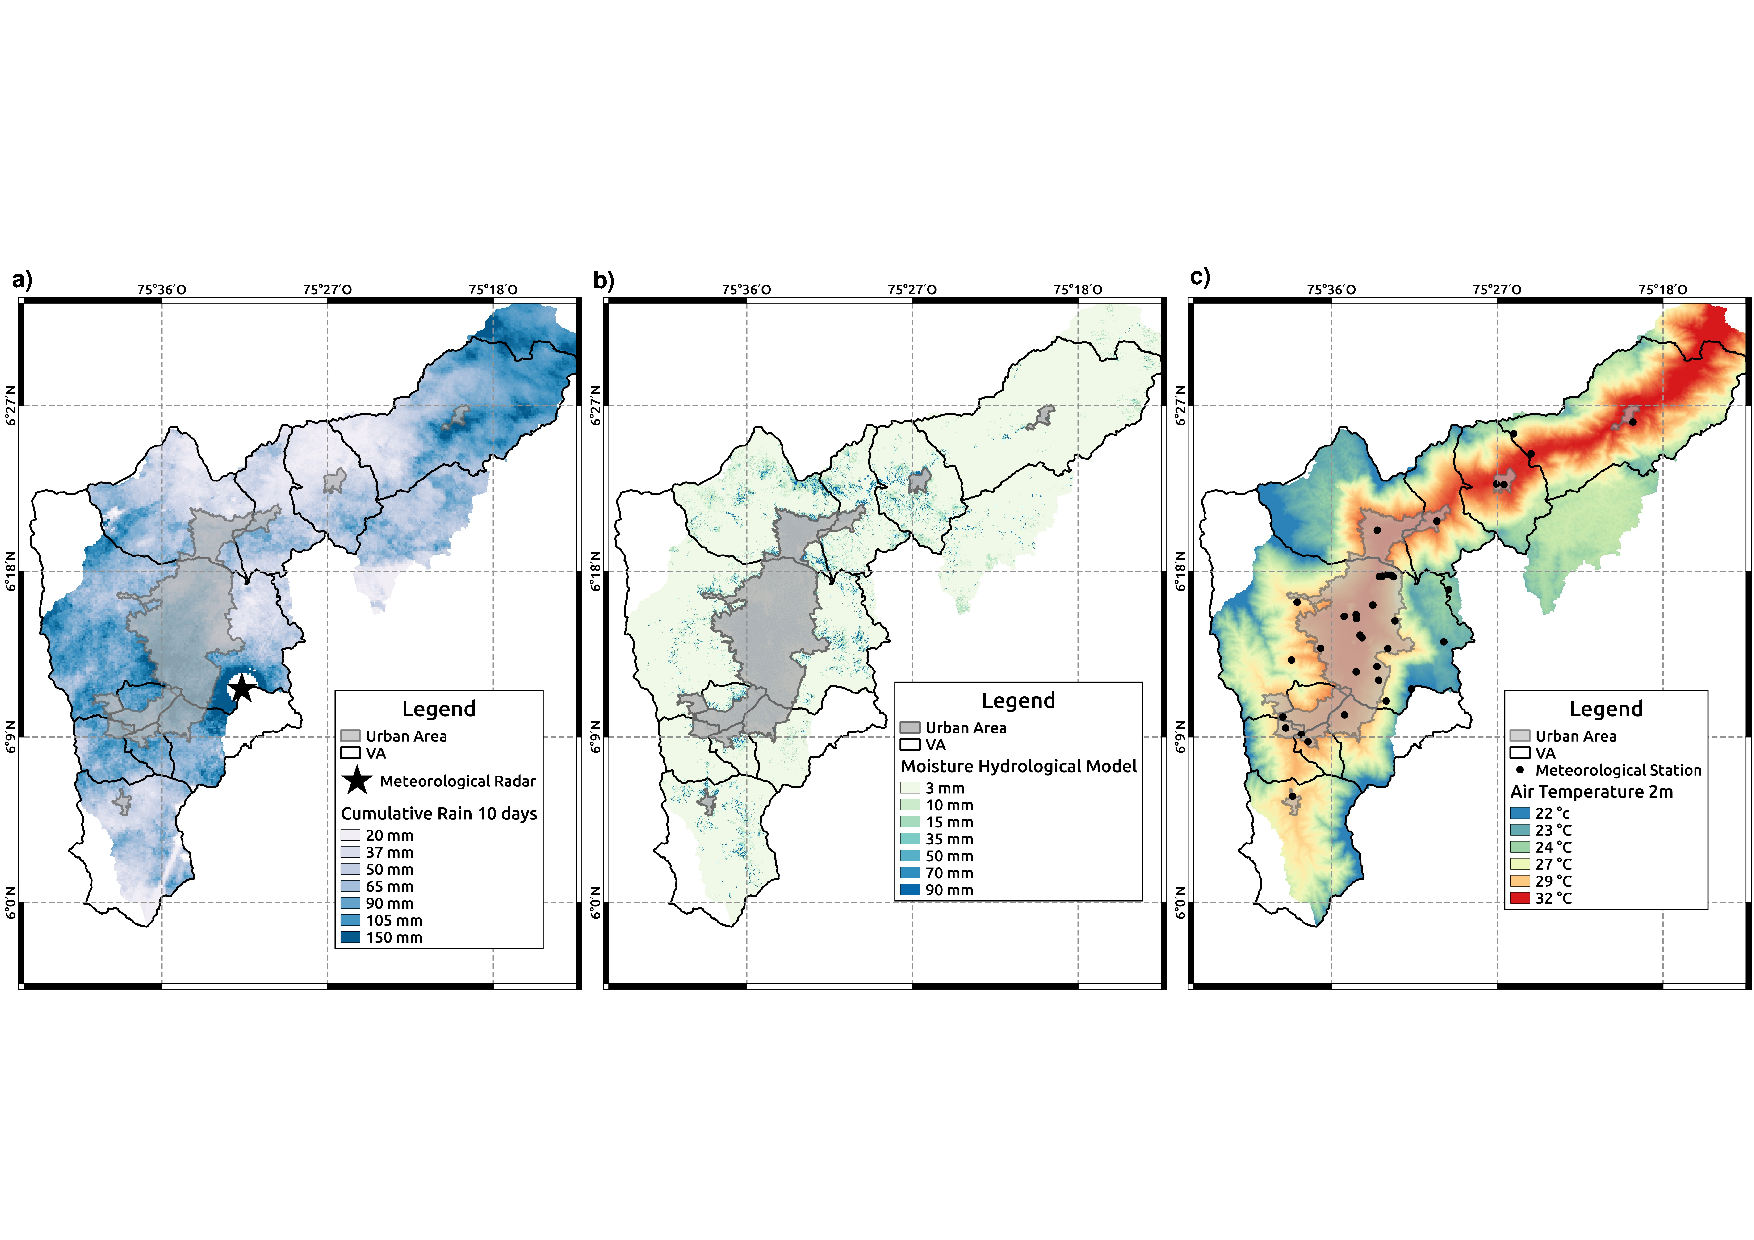
\includegraphics[width=1.0\linewidth]{Figuras/dynamic_composition1.pdf}
  \caption{Dynamic layer. Cumulative rain 10 days, soil moisture and surface temperature.}
  \label{fig:dynamicLayers}
\end{figure*}

In the Table \ref{Tab:info_all} we show a summary of the information used for the development of the strategy and the model. Both, temporal and spatial resolution change from variable to variable (column 3 at Table \ref{Tab:info_all}), however, when used, the temporal scale is fixed to 1 hour and the spatial scale to 60m. 

\begin{table}[!h]
\label{Tab:info_all}
\caption{Information}
\begin{tabular}{| c | c | c | c | c |}
\hline
\textbf{Parameter} & \textbf{Type} & \textbf{Scale} & \textbf{Resolution} & \textbf{Source} \\
\hline

Surface Temperature  (2m) & WRF Model & 2 km & Hourly & SIATA \\ \hline
Air Temperature  & Recorded & Punctual Value  & 1 Minute & SIATA \\ \hline
Rain 10 days & Radar  & 150 m & 5 minutes & SIATA \\ \hline
Soil Moisture & Map & 60m & 5 minutes & SIATA \\ \hline
Land Use & Map & 50 cm & Fixed & SIATA \\ \hline
Wildfire Records & Database &  Events & Fixed & Fire Brigades\\
Recorded wildfires & Database & Events & SIATA \\
\hline

\end{tabular}
\end{table}